\documentclass[a4paper,12pt]{article}
\usepackage[utf8]{inputenc}
\usepackage[ngerman]{babel}
\usepackage{amsmath}
\usepackage{wrapfig} 
\usepackage{enumitem}
\usepackage{amsfonts}
\usepackage{graphicx}
\usepackage{xcolor}
\usepackage{geometry}
\usepackage[most]{tcolorbox}
\geometry{margin=2.5cm}

  \tcbset{
   colback=gray!5,
   colframe=gray!50,
   coltitle=black,
   colbacktitle=white,
   boxrule=0.5pt,
   arc=4pt,
   left=6pt,
   right=6pt,
   top=4pt,
   bottom=4pt,
   fonttitle=\bfseries,
 }



\title{Numerische Betrachtung der impliziten Volatilität}
\author{Alexandros Apostolidis}
\date{02.06.2025}

\begin{document}
\maketitle


\section*{1. Motivation und Einordnung}

\subsection*{1.1 Was ist die implizite Volatilität (IV)?}
Die implizite Volatilität (IV) ist ein zentrales Konzept in der Optionsbewertung: Sie reflektiert die vom Markt erwartete Schwankungsbreite eines Basiswerts, ohne direkt beobachtbar zu sein. Stattdessen wird sie aus beobachteten Optionspreisen rückgerechnet.

Im Gegensatz zur historischen Volatilität, die auf vergangenen Kursbewegungen basiert, liefert die IV ein zukunftsgerichtetes Maß für Unsicherheit. Sie ist entscheidend für eine Vielzahl praktischer Anwendungen – vom Risk Management über Volatilitätsarbitrage bis zur Modellkalibrierung in der Derivatebewertung.

\subsection*{1.2 Warum ist sie entscheidend für Pricing, Risk Management und Marktstruktur?}
Die IV ist fundamentaler Bestandteil von Optionsbewertung, Hedging und Risikomanagement. Sie wird zur Kalibrierung von Derivatemodellen, zur Einschätzung von Markterwartungen und als Signal in Handelsstrategien verwendet. In Volatilitätsarbitrage und der Analyse von Volatility Surfaces spielt sie eine zentrale Rolle.

\subsection*{1.3 Warum ist numerische Berechnung überhaupt notwendig?}
Die Black-Scholes-Gleichung lässt sich nicht analytisch nach der Volatilität auflösen. Die IV ist also die Lösung eines nichtlinearen Inversionsproblems. In der Praxis wird sie mithilfe numerischer Verfahren wie Brent’s Method oder Newton-Verfahren berechnet. Dabei treten Probleme wie schlechte Konditionierung oder Nichtkonvergenz auf – insbesondere bei exotischen Marktbedingungen oder illiquiden Optionen.


\clearpage
\section*{2. Mathematische Grundlagen}

\subsection*{2.1 Die Black-Scholes-Gleichung als Vorwärtsmodell}
Die Black-Scholes-Gleichung liefert den theoretischen Optionspreis $C$ als Funktion der Parameter Spotpreis $S$, Strike $K$, Restlaufzeit $T$, Zinssatz $r$ und Volatilität $\sigma$:

\[
C = BS(S, K, T, r, \sigma)
\]

Alle Größen bis auf $\sigma$ sind beobachtbar oder modellseitig gesetzt. Die Volatilität ist der freie Parameter, der aus Marktpreisen rückgeschlossen wird.

\subsection*{2.2 Inversionsproblem: Zielgröße implizite Volatilität}
Gesucht ist diejenige Volatilität $\sigma^*$, für die der theoretische Preis dem beobachteten Marktpreis entspricht:

\[
BS(S, K, T, r, \sigma^*) = C_{\text{markt}}
\]

Da $BS(\cdot)$ in $\sigma$ nicht analytisch invertierbar ist, handelt es sich um ein nichtlineares numerisches Problem.

\subsection*{2.3 Formulierung als Nullstellenproblem}
Die Inversion kann formuliert werden als Nullstellenproblem einer Zielfunktion:

\[
f(\sigma) := BS(S, K, T, r, \sigma) - C_{\text{markt}} = 0
\]

Diese Funktion ist für Standardparameter monoton wachsend in $\sigma$ und stetig. Dies ermöglicht robuste numerische Verfahren zur Bestimmung der Nullstelle.


\subsection*{2.4 Praktische Herausforderungen}
Trotz der theoretischen Eigenschaften treten in der Praxis mehrere Probleme auf:

\begin{itemize}
  \item Nichtkonvergenz bei extremen Parametern (z.\,B. sehr tief OTM)
  \item Instabilität bei geringer Vega $\left( \frac{\partial C}{\partial \sigma} \approx 0 \right)$
  \item Diskrete Preisdaten und Bid/Ask-Spannen
\end{itemize}

Die numerische Umsetzung muss daher sowohl robust als auch effizient gestaltet sein.
\begin{tcolorbox}[title=Ökonomische Interpretation von Vega $\left( \frac{\partial C}{\partial \sigma} \right)$]
    Die Vega misst die Sensitivität des Optionspreises $C$ gegenüber kleinen Änderungen der Volatilität $\sigma$:
    
    \[
    \text{Vega} = \frac{\partial C}{\partial \sigma}
    \]
    
    Im Kontext des Newton-Verfahrens spielt sie eine zentrale Rolle als Nenner in der Iterationsformel. Ein hoher Vega-Wert bedeutet, dass kleine Volatilitätsänderungen zu merklichen Preisänderungen führen – was die Inversion stabil und schnell konvergierend macht.
    
    Umgekehrt gilt: Ist Vega klein, so reagiert der Preis kaum auf Änderungen in $\sigma$, was numerisch instabile Updates verursacht. Besonders kritisch sind:
    \begin{itemize}
      \item Optionen tief aus dem Geld
      \item Sehr kurze Restlaufzeiten
      \item Märkte mit geringer impliziter Volatilität
    \end{itemize}
    
    Ökonomisch deutet eine geringe Vega darauf hin, dass der Markt einer Volatilitätsänderung in diesem Strike/Term-Segment wenig Gewicht beimisst – z.\,B. bei illiquiden Optionen oder hoher Sicherheit über das künftige Kursverhalten.
    \end{tcolorbox}


\section*{3. Numerische Inversion und Implementierung}

\subsection*{3.1 Numerische Verfahren zur Inversion}

Da die Black-Scholes-Gleichung in $\sigma$ nicht analytisch invertierbar ist, kommen numerische Nullstellensuchverfahren zum Einsatz.

\paragraph{Brent's Method} kombiniert Bisektion, Sekantenmethode und inverse Parabelinterpolation. Sie ist robust gegenüber schlechter Startwerte und benötigt keine Ableitung der Zielfunktion.

\paragraph{Newton-Verfahren} nutzt die erste Ableitung (Vega) zur Konvergenzbeschleunigung:

\[
\sigma_{n+1} = \sigma_n - \frac{f(\sigma_n)}{f'(\sigma_n)} = \sigma_n - \frac{BS(\sigma_n) - C_{\text{markt}}}{\text{Vega}(\sigma_n)}
\]

\textbf{Problem:} Bei geringer Vega oder schlechter Startnähe kann das Verfahren divergieren oder instabil werden.

\paragraph{Abbruchkriterien:}
Typischerweise gilt:

\[
|f(\sigma_n)| < \varepsilon \quad \text{mit z.\,B. } \varepsilon = 10^{-6}
\]

Zusätzlich sollte $\sigma_n$ in einem stabilen Intervall $[\sigma_{\min}, \sigma_{\max}]$ bleiben (z.\,B. $[0.01, 2.0]$), um numerische Ausreißer zu vermeiden.

\subsection*{3.2 Beispielrechnung: Konvergente Lösung und Vega-Abhängigkeit}

\textbf{Gegeben:}
\begin{itemize}
  \item Spotpreis: $S = 100$
  \item Strike: $K = 105$
  \item Restlaufzeit: $T = 0{,}25$
  \item Zinssatz: $r = 0{,}01$
  \item Marktpreis der Option: $C_{\text{markt}} = 2{,}35$
\end{itemize}

\textbf{Ziel:} Bestimme $\sigma^*$ mit $BS(...) = 2{,}35$.

\textbf{Lösung via Brent:}  
Nach 6 Iterationen ergibt sich:

\[
\sigma^* = 0{,}2741 \quad \text{mit } \text{Vega} \approx 0{,}112
\]

\begin{figure}[h]
  \centering
  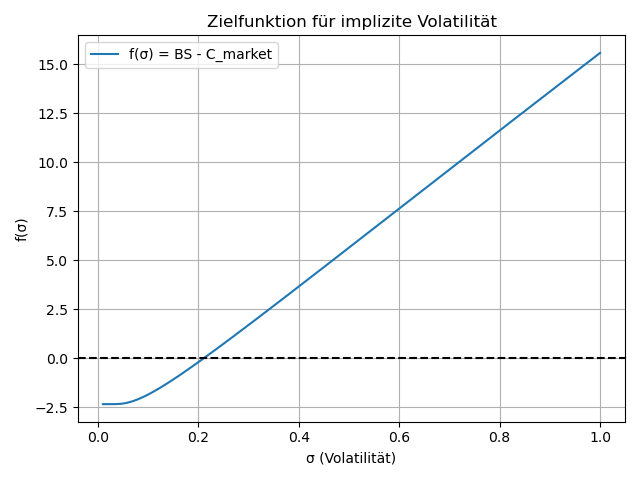
\includegraphics[width=0.6\textwidth]{iv_root_example.png}
  \caption{Verlauf der Zielfunktion \( f(\sigma) = BS(\sigma) - C_{\text{markt}} \). Die implizite Volatilität \( \sigma^* \) ergibt sich als Nullstelle dieser Funktion – hier bei etwa 0{,}274. Die Monotonie erleichtert den Einsatz numerischer Verfahren wie Brent's Method.}
\end{figure}

\textbf{Interpretation:}  
Ein kleiner Vega-Wert führt zu schlechterer Konditionierung. Die Inversion ist empfindlich gegenüber numerischem Rauschen, z.\,B. durch Bid/Ask-Spread oder Modellabweichungen.

\textbf{Ökonomische Interpretation:}  
Die berechnete Volatilität \(\sigma^* = 0{,}2741\) repräsentiert die vom Markt implizit erwartete Schwankungsintensität des Basiswerts bis zum Laufzeitende – hier über einen Zeitraum von 3 Monaten. Da der Strike mit 105 leicht über dem Spotpreis von 100 liegt, reflektiert \(\sigma^*\) speziell die Unsicherheit in der rechten Flanke der Verteilung (Out-of-the-Money Calls). Höhere Werte deuten auf ein Risikoanstiegsszenario oder eine erhöhte Prämie für Upside Exposure hin.



\subsection*{3.3 Fehlerquellen und Regularisierung}

\begin{itemize}
  \item Ungenaue oder veraltete Marktpreise → Verschiebung der Lösung
  \item Division durch numerisch kleine Vega
  \item Instabilität bei $\sigma < 0.01$ oder $\sigma > 2.0$
\end{itemize}

\paragraph{Gegenmaßnahmen:}
\begin{itemize}
  \item Eingeschränktes Intervall $[\sigma_{\min}, \sigma_{\max}]$
  \item Mindestvega-Schwelle: $\text{Vega} > \delta$
  \item Verwendung von Bid/Ask-Mittelwerten als $C_{\text{markt}}$
\end{itemize}

\subsection*{Konvergenz und Performance}
Brent konvergiert superlinear (i.\,d.\,R. in 5–7 Iterationen). Alternativen wären Newton-Verfahren:

\[
\sigma_{n+1} = \sigma_n - \frac{f(\sigma_n)}{f'(\sigma_n)}
\quad \text{mit} \quad f'(\sigma) = \text{Vega}
\]

→ aber instabil, wenn Vega klein.

\subsection*{3.4 Implementierung in der Datenpipeline}

Zur Laufzeit werden IV-Werte automatisiert aus Marktpreisen berechnet. Dabei:

\begin{itemize}
  \item Outlier-Clipping $[0.01, 2.0]$
  \item Mindestpreisgrenze $C_{\text{markt}} > 0.05$
  \item Bid/Ask-Mittelwert als robuste Eingabe
  \item Fallback auf vorherigen IV-Wert bei Nichtkonvergenz
\end{itemize}
\begin{tcolorbox}[colback=yellow!5!white,colframe=yellow!80!black,title=Warnhinweis: Newton-Verfahren kann instabil werden]    Das Newton-Verfahren ist ein schnelles, aber sensibles Optimierungsverfahren. In der IV-Berechnung kann es versagen, wenn:
    \begin{itemize}
      \item die Zielfunktion flach ist (z.\,B. bei geringer Vega),
      \item der Startwert zu weit vom Ziel entfernt liegt,
      \item die Ableitung numerisch instabil wird (z.\,B. bei Preisdiskontinuitäten oder illiquiden Optionen).
    \end{itemize}
    In solchen Fällen kann es zu Divergenz oder Oszillation kommen. Deshalb wird in der Praxis oft ein hybrider Ansatz verwendet: Zunächst eine robuste Methode wie Brent oder Bisection, danach ggf. ein Newton-Finetuning.
    \end{tcolorbox}
    
    \vspace{1em}

\clearpage
\section*{4. Erweiterung durch stochastische Modelle}

\subsection*{4.1 Motivation und Abweichung vom Black-Scholes-Modell}
Die klassische Black-Scholes-Theorie geht von konstanter Volatilität aus – eine Annahme, die in der Realität oft verletzt wird. Stochastische Volatilitätsmodelle wie Heston oder SABR berücksichtigen die zufällige Natur der Volatilität selbst und erlauben damit eine realistischere Bewertung und IV-Schätzung.

\subsection*{4.2 Einfluss stochastischer Volatilität auf die IV-Bestimmung}
Stochastische Volatilitätsmodelle erzeugen eine Streuung der Optionspreise für gegebene Marktparameter. In einer Monte-Carlo- oder PDE-basierten Simulation ergeben sich Erwartungswerte und Varianzen für den Optionspreis als Funktion von Spotpreis und Zeit.

\begin{figure}[h]
    \centering
    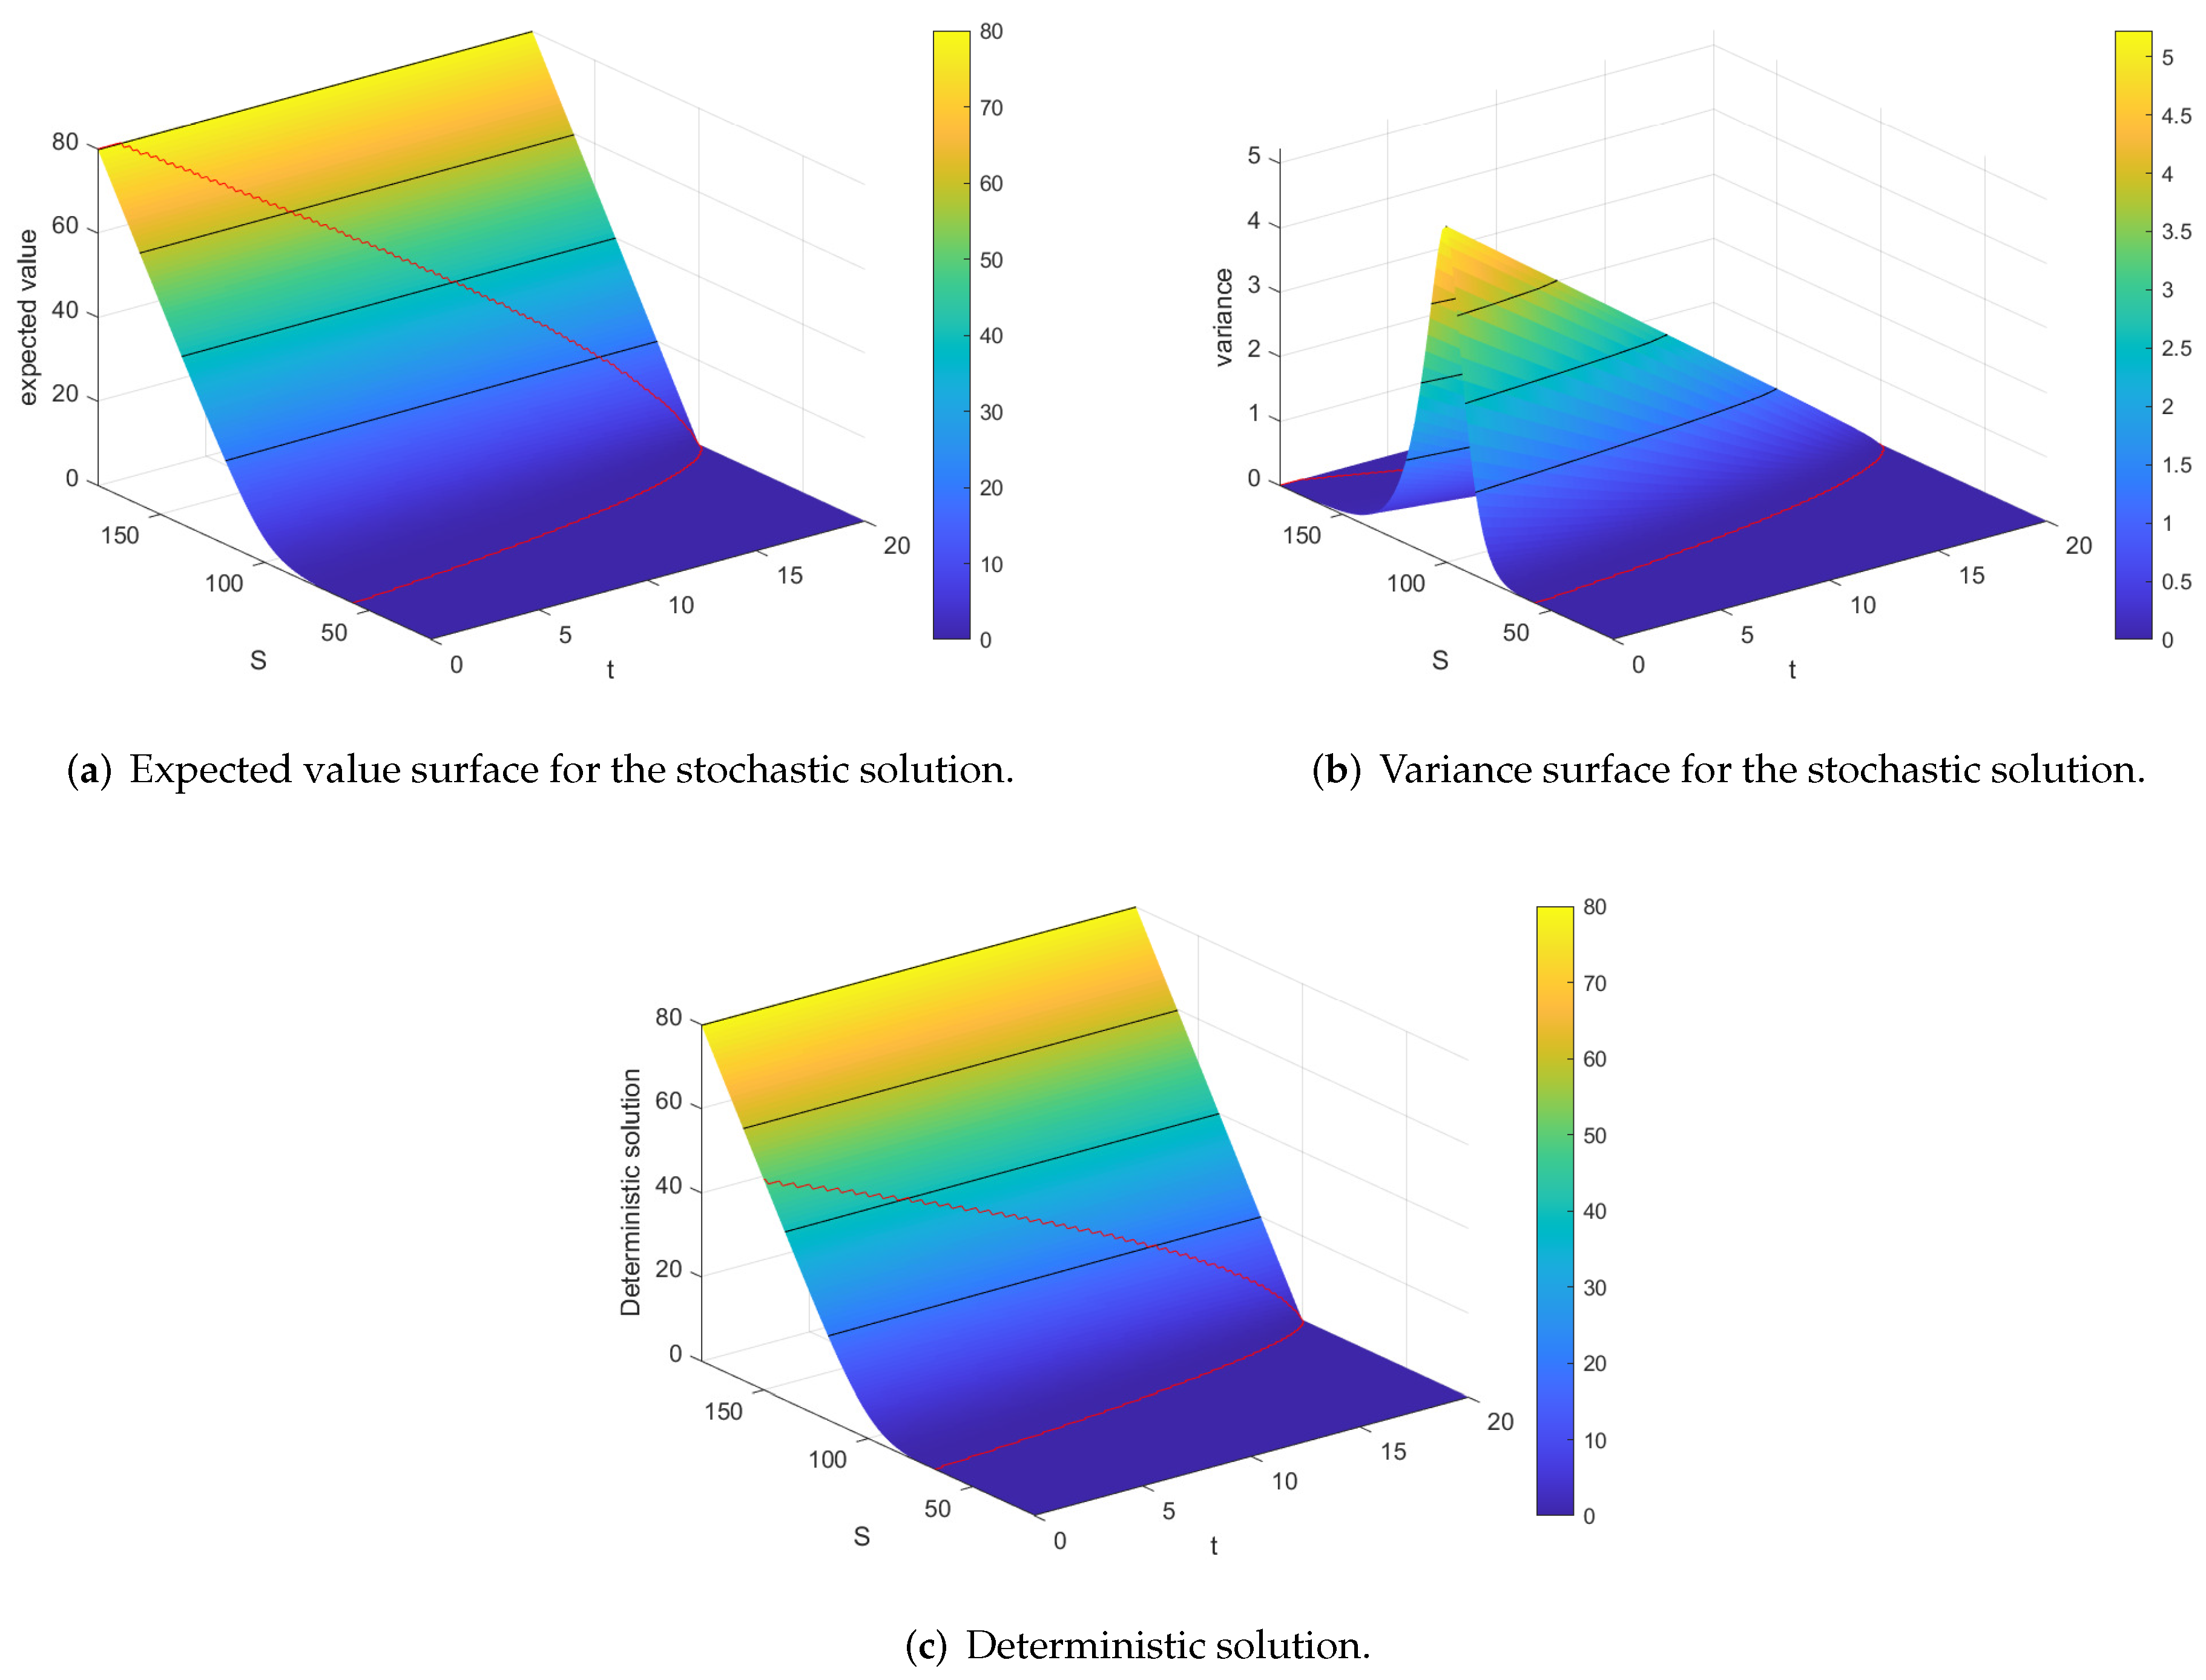
\includegraphics[width=0.85\textwidth]{fig2.png} % oder mathematics-10-00489-g001.png
    \caption{Simulierte Preisoberflächen unter stochastischer Volatilität: (a) Erwartung, (b) Varianz, (c) deterministische Lösung. Die Streuung im Preis beeinflusst die Stabilität der IV-Inversion.}
\end{figure}

Diese Preisstreuung bedeutet, dass sich für identische Marktparameter nicht ein einzelner Optionspreis, sondern eine Preisverteilung ergibt. Daraus folgt: Es gibt keine eindeutige implizite Volatilität mehr, sondern eine IV-Verteilung. In der Praxis zeigt sich dies durch:

\begin{itemize}
  \item Verrauschte IV-Schätzungen und erhöhte Streuung.
  \item Stochastische Inputs in der numerischen Inversion → größere Unsicherheit.
  \item Instabile oder springende IV-Werte bei Marktstress oder illiquiden Strikes.
\end{itemize}



% 4.3
\subsection*{4.3 Numerische Konsequenzen stochastischer Volatilität}

Die Modellierung stochastischer Volatilität führt zu einer Preisverteilung statt eines eindeutigen Optionspreises. Das erschwert die IV-Bestimmung numerisch erheblich – insbesondere in Regionen mit geringer Sensitivität.

\begin{itemize}
  \item In Regionen mit hoher Preisvarianz oder geringer Vega wird die Inversion instabil.
  \item Kleine Inputabweichungen (z.\,B. durch Bid/Ask-Spannen) wirken sich überproportional auf das Ergebnis aus.
  \item Klassische Verfahren wie das Newton-Verfahren versagen hier häufig aufgrund schlechter Kondition.
\end{itemize}
Diese Effekte stellen eine erhebliche Herausforderung für die numerische Bestimmung der IV dar.

% 4.4
\subsection*{4.4 Vega-Sensitivität im Strike–Laufzeit-Raum}

Um diese Sensitivitätsstruktur zu analysieren, betrachten wir die Vega-Verteilung im Strike–Laufzeit-Raum unter einem Heston-Modell:

\begin{figure}[h]
    \centering
    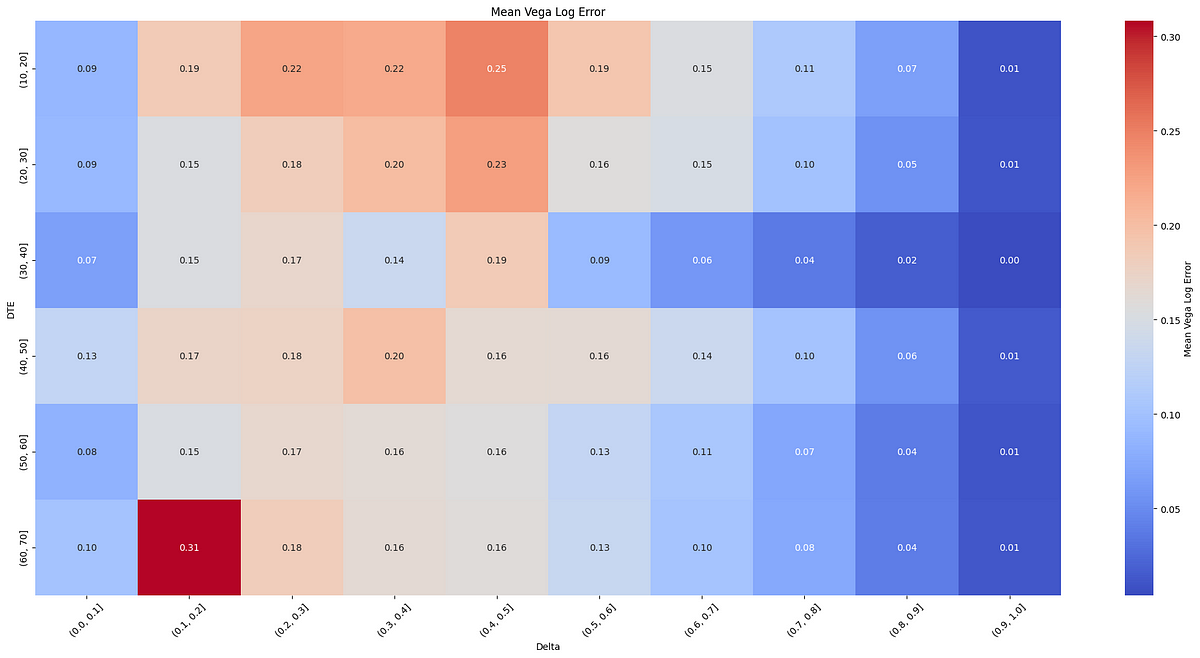
\includegraphics[width=0.85\textwidth]{heston_vega_heatmap.png}
    \caption{Vega-Heatmap unter einem Heston-Modell: Niedrige Vega-Werte (blau) markieren Regionen mit hoher numerischer Instabilität. Besonders kritisch sind kurze Laufzeiten und weit aus dem Geld liegende Optionen.}
\end{figure}

Die Grafik zeigt: In Zonen geringer Vega ist die numerische Inversion schlecht konditioniert – kleine Fehler im Marktpreis führen zu großen Fehlern in der geschätzten IV. Besonders betroffen sind:

\begin{itemize}
  \item Optionen mit kurzer Restlaufzeit
  \item Stark OTM-Optionen
  \item Märkte mit hoher Unsicherheit oder geringer Liquidität
\end{itemize}

Daraus folgt: In diesen Regionen ist eine robuste Fehlerbehandlung (z.\,B. Intervallbeschränkung, Mindestvega) essenziell.

% 4.5
\subsection*{4.5 Praktische Maßnahmen bei numerischer Instabilität}

\begin{itemize}
  \item Dynamische Intervallwahl für $\sigma_{\min}, \sigma_{\max}$ je nach Marktvolatilität
  \item Einführen einer Mindest-Vega-Schranke: $\text{Vega} > \delta$
  \item Robuste Verfahren mit Fallbacks bei Nichtkonvergenz
\end{itemize}
Diese lokalen Instabilitäten schlagen sich in der Struktur ganzer IV-Surfaces nieder.



% --- NEUER ABSCHNITT 5 ---
\section*{5. IV-Surfaces und dynamische Modellierung}

\subsection*{5.1 Geometrie und Struktur der IV-Surface}

Implizite Volatilität ist keine eindimensionale Kennzahl, sondern hängt maßgeblich vom Strike $K$ und der Restlaufzeit $T$ ab. Daraus ergibt sich eine IV-Oberfläche:
\[
\sigma_{\text{impl}} = \sigma(K, T)
\]
In der Praxis wird diese Surface zusätzlich für verschiedene Underlyings und über die Zeit $t$ beobachtet, woraus sich eine 4D-Struktur ergibt:
\[
\sigma_{\text{impl}} = \sigma(K, T; \text{Asset}, t)
\]

\paragraph{Typische Struktureigenschaften:}
\begin{itemize}
  \item \textbf{Volatility Smile / Skew:} Unterschiedliches Verhalten für ITM/ATM/OTM-Optionen.
  \item \textbf{Termstruktur:} Kurz- vs. langfristige Volatilität weichen oft deutlich ab.
  \item \textbf{Clustering:} Assets mit ähnlicher Risikostruktur zeigen vergleichbare Oberflächenmuster.
\end{itemize}


\begin{wrapfigure}{R}{0.5\textwidth}
  \centering
  \vspace{-1em}
  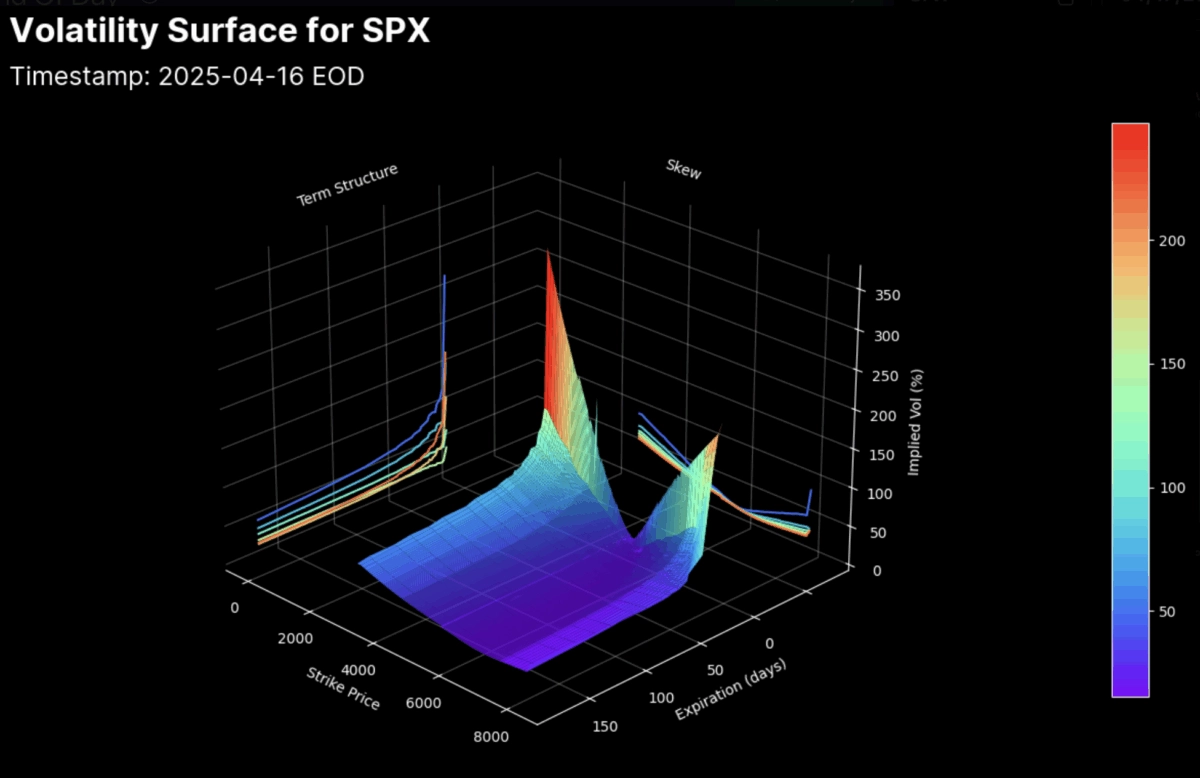
\includegraphics[width=0.4\textwidth]{VS3d.png}
  \caption{IV-Surface für den SPX am 16.04.2025.}
  \vspace{-1em}
\end{wrapfigure}

\paragraph{Visualisierung:}
Die implizite Volatilitätsoberfläche kann auf verschiedene Weise visualisiert werden. Häufig verwendet werden Heatmaps, die für eine feste Laufzeit oder einen bestimmten Strike-Bereich die Volatilitätsverteilung zweidimensional darstellen. Eine weitere gebräuchliche Methode sind 3D-Plots, bei denen die IV über der Strike-Laufzeit-Ebene kontinuierlich aufgetragen wird. Diese Darstellungen ermöglichen es, Muster wie Skews, Smiles oder abrupte Strukturbrüche visuell zu erfassen und zu interpretieren.
\clearpage

\subsection*{5.2 Zeitliche Dynamik der IV-Oberfläche}

Die IV-Surface ist hochdynamisch und reagiert sensibel auf Marktveränderungen:
\begin{itemize}
  \item \textbf{Ereignisgetrieben:} Earnings, Notenbanksitzungen, geopolitische Schocks.
  \item \textbf{Gleitende Regimewechsel:} Übergang von ruhigen zu volatilen Marktphasen.
  \item \textbf{Mean-Reversion vs. Shock-Propagation:} IV kehrt häufig zu Mittelwerten zurück, propagiert aber auch neue Risikoerwartungen.
\end{itemize}

Solche Dynamiken zeigen, dass IV nicht nur Risiko misst, sondern auch Markterwartungen und Unsicherheit über Zeit enkodiert.
\subsection*{5.3 Modellierung der IV-Dynamik}

Die Bewegung der IV-Surface über die Zeit spiegelt Veränderungen in Marktstimmung, Risikopräferenzen und Ereignisrisiken wider. Um diese Dynamik systematisch zu erfassen und prognostizierbar zu machen, werden strukturierte Modellierungsansätze benötigt. Zwei besonders verbreitete Methoden sind die Principal Component Analysis (PCA) und der Kalman-Filter. Beide verfolgen unterschiedliche Ziele: Während PCA auf strukturelle Zerlegung abzielt, modelliert der Kalman-Filter die zeitliche Entwicklung latenter Zustände.

\subsubsection*{5.3.1 PCA: Strukturzerlegung}

Die Principal Component Analysis reduziert die hochdimensionale IV-Oberfläche auf wenige dominante Bewegungsmuster:
\begin{itemize}
  \item \textbf{Level:} Verschiebung des allgemeinen Volatilitätsniveaus
  \item \textbf{Slope:} Änderung des Skews über den Strike
  \item \textbf{Curvature:} Intensität von Smile-Strukturen
\end{itemize}

Jede IV-Surface kann so als Linearkombination dieser orthogonalen Komponenten rekonstruiert werden. Das erlaubt nicht nur visuelle Kompression, sondern auch eine klare Interpretation von Volatilitätsänderungen.\\



\noindent
\begin{minipage}[t]{0.48\textwidth}
\begin{tcolorbox}[colback=blue!5!white, colframe=blue!75!black, title=Vorteile]
\begin{itemize}
  \item Intuitive Interpretation der Hauptmodi
  \item Hohe Recheneffizienz
  \item Nützlich zur Dimensionsreduktion und Feature-Extraktion
\end{itemize}
\end{tcolorbox}
\end{minipage}
\hfill
\begin{minipage}[t]{0.48\textwidth}
\begin{tcolorbox}[colback=red!5!white, colframe=red!75!black, title=Grenzen]
\begin{itemize}
  \item Keine explizite Zeitmodellierung
  \item Stationaritätsannahme notwendig
  \item Sensitiv gegenüber strukturellen Brüchen oder Ausreißern
\end{itemize}
\end{tcolorbox}
\end{minipage}

\subsubsection*{5.3.2 Kalman-Filter: Dynamische Rekonstruktion}

Der Kalman-Filter bietet ein rekursives Framework zur Schätzung zeitlich variierender Zustände. Im Kontext der IV-Surface wird er oft auf die projizierten PCA-Komponenten angewendet, um deren Entwicklung als latente Prozesse zu modellieren.

\begin{itemize}
  \item \textbf{Zustandsraum-Modell:} Trennung von Systemdynamik und Beobachtung
  \item \textbf{Rekursive Schätzung:} Integration neuer Datenpunkte in Echtzeit
  \item \textbf{Rauschanpassung:} Berücksichtigung von Beobachtungs- und Prozessunsicherheit
\end{itemize}


\noindent
\begin{minipage}[t]{0.48\textwidth}
\begin{tcolorbox}[colback=blue!5!white, colframe=blue!75!black, title=Vorteile]
\begin{itemize}
  \item Echtzeitfähige Modellierung mit Unsicherheitsquantifizierung
  \item Gute Prognoseeigenschaften
  \item Robust gegenüber Datenlücken oder verrauschten Eingaben
\end{itemize}
\end{tcolorbox}
\end{minipage}
\hfill
\begin{minipage}[t]{0.48\textwidth}
\begin{tcolorbox}[colback=red!5!white, colframe=red!75!black, title=Grenzen]
\begin{itemize}
  \item Höherer Implementierungsaufwand
  \item Kalibrierung sensibel auf Modellannahmen
  \item Linearisierung notwendig bei nichtlinearen Prozessen
\end{itemize}
\end{tcolorbox}
\end{minipage}

\subsubsection*{5.3.3 Kombination beider Verfahren}

In der Praxis ergibt sich ein synergetischer Vorteil durch die Kombination beider Ansätze:

\begin{itemize}
  \item \textbf{PCA:} Reduktion der komplexen Surface auf wenige erklärende Faktoren
  \item \textbf{Kalman-Filter:} Dynamische Modellierung und Glättung dieser Faktoren über die Zeit
\end{itemize}

Solche hybriden Modelle erlauben eine robuste, skalierbare und adaptiv erweiterbare IV-Modellierung. Sie sind insbesondere nützlich für:
\begin{itemize}
  \item \textit{Forecasting}: Vorhersage zukünftiger IV-Strukturen
  \item \textit{Stress-Tests}: Szenarioanalyse unter hypothetischen Shifts
  \item \textit{Risikoüberwachung}: Detektion von Regimewechseln
\end{itemize}
\clearpage

\subsection*{5.4 Prognose und Szenarienanalyse}

Neben der Beschreibung und Reduktion der IV-Surface ist auch deren prognostische Nutzung zentral. Dazu existieren mehrere Klassen von Modellen, von regelbasierten Shift-Strukturen bis hin zu datengesteuerten Lernverfahren.

\subsubsection*{5.4.1 Shift-Modelle}

Ein klassischer Ansatz ist die Modellierung von Szenarien durch gezielte Shifts in der IV-Surface:
\begin{itemize}
  \item \textbf{Level-Shift:} gleichmäßige Anhebung oder Absenkung der gesamten Surface
  \item \textbf{Slope-Shift:} Veränderung der Steigung (z.\,B. steilerer Skew)
  \item \textbf{Curvature-Shift:} Betonung oder Glättung von Smile-Strukturen
\end{itemize}

Diese Shifts lassen sich auch mit PCA-Komponenten überlagern, um hypothetische Marktbewegungen durchzuführen, etwa:
\begin{itemize}
  \item Anstieg der Unsicherheit vor einem Earnings-Termin
  \item Rückbildung einer IV-Anomalie nach einem Event
\end{itemize}

\subsubsection*{5.4.2 Datengestützte Prognoseverfahren}

Für die zeitliche Prognose der IV-Surface kommen zunehmend datengetriebene Modelle zum Einsatz:

\begin{itemize}
  \item \textbf{Zeitreihenmodelle:} ARIMA, GARCH, State-Space-Modelle
  \item \textbf{Maschinelles Lernen:} Recurrent Neural Networks (RNNs), Transformer, Gaussian Processes
  \item \textbf{Latent Embeddings:} Nutzung von VAE oder Autoencoder-Architekturen zur IV-Kodierung
\end{itemize}

Diese Modelle können historische Surface-Zeitreihen analysieren, Muster extrahieren und zukünftige Bewegungen prognostizieren. Besonders Transformer-basierte Systeme zeigen hohes Potenzial bei strukturierter Vorhersage über mehrere Dimensionen.

\subsubsection*{5.4.3 Kombination mit Risikoszenarien}

In der Praxis werden Shift-Modelle und ML-Prognosen häufig kombiniert:

\begin{itemize}
  \item \textbf{Baseline:} datengestützte Forecasts
  \item \textbf{Overlay:} manuelle Stress-Szenarien zur Robustheitsanalyse
\end{itemize}

Solche hybriden Ansätze erlauben die Planung unter Unsicherheit – insbesondere bei portfoliobasierter Optionsbewertung oder regulatorischen Stresstests.


\subsection*{5.5 Limitations und Modellrisiken}

Trotz der Fortschritte in der Modellierung impliziter Volatilität bleiben grundlegende Limitationen bestehen – sowohl theoretischer als auch praktischer Natur.

\subsubsection*{5.5.1 Theoretische Beschränkungen}

\begin{itemize}
  \item \textbf{Modellannahmen:} Sowohl Black-Scholes als auch stochastische Modelle beruhen auf idealisierten Annahmen (z.\,B. stetige Handelsbarkeit, konstante Parameter, keine Arbitrage), die in der Realität oft verletzt sind.
  \item \textbf{Nicht-Eindeutigkeit der IV:} Bei stochastischer Volatilität oder diskreter Preisdatenlage existiert keine eindeutige Lösung für die IV – insbesondere bei geringem Vega oder illiquiden Optionen.
  \item \textbf{Dimensionsreduktion:} Verfahren wie PCA setzen auf lineare Strukturen. Nichtlineare Dynamiken oder Interaktionen zwischen Dimensionen können dadurch verzerrt werden.
\end{itemize}

\subsubsection*{5.5.2 Numerische Herausforderungen}

\begin{itemize}
  \item \textbf{Instabile Inversion:} Die numerische Lösung ist besonders in extremen Marktsegmenten (z.\,B. OTM, kurze Laufzeiten) anfällig für Instabilität und Nichtkonvergenz.
  \item \textbf{Sensitivität gegenüber Preisfehlern:} Kleine Störungen im Optionspreis führen bei geringer Vega zu großen Schätzfehlern in der IV.
  \item \textbf{Interpolation/Glättung:} Die Konstruktion glatter IV-Surfaces erfordert Interpolation, was bei stochastischem Input zu Artefakten führen kann.
\end{itemize}

\subsubsection*{5.5.3 Modellrisiken in der Anwendung}

\begin{itemize}
  \item \textbf{Falsche Modellwahl:} Ein ungeeignetes Modell (z.\,B. konstante Volatilität bei starkem Smile) führt zu systematischen Fehlschätzungen.
  \item \textbf{Überanpassung:} Hochparametrische Modelle können historische Daten gut erklären, versagen aber bei Prognosen.
  \item \textbf{Regimewechsel:} Plötzliche Marktbrüche machen zuvor kalibrierte Modelle unbrauchbar. Besonders datengetriebene Verfahren leiden unter strukturellen Brüchen.
\end{itemize}

\subsubsection*{Fazit}

Die Wahl und Kalibrierung von IV-Modellen ist stets mit Unsicherheit behaftet. Deshalb ist es essenziell, Sensitivitätsanalysen, Fallback-Mechanismen und regelmäßige Modellvalidierung zu integrieren. IV-Modelle sollten als adaptive Approximation verstanden werden – nicht als deterministische Wahrheiten.

\section*{6. Anwendungen und Bedeutung der impliziten Volatilität}
Nach der formalen Herleitung und numerischen Lösung der IV wenden wir uns nun der praktischen Bedeutung dieser Größe in verschiedenen Anwendungsfeldern zu.
\subsection*{6.1 Optionsbewertung und Derivatepricing}
Die IV ist zentral für die Bewertung von Optionen und derivativen Finanzinstrumenten. In praxistauglichen Modellen (u.\,a. Heston, SABR) wird sie als Basis für die Kalibrierung genutzt. Ohne IV wäre eine marktnahe Preisstellung nicht möglich.

\subsection*{6.2 Risikomanagement und Sensitivitätsanalyse}
Implizite Volatilität beeinflusst maßgeblich die Sensitivitätskennzahlen (Greeks), insbesondere Vega. Änderungen in der IV wirken sich direkt auf Risikoprofile und Hedging-Strategien aus. In der Praxis wird IV zur Risikoklassifizierung von Positionen verwendet.

\subsection*{6.3 Marktsentiment und Prognoseindikator}
Ein Anstieg der IV wird häufig als Zeichen für erhöhte Unsicherheit oder erwartete Marktturbulenzen interpretiert. Der VIX („Volatility Index“) fungiert als „Angstbarometer“. IV-Zeitreihen werden oft zur Einschätzung von Extremrisiken oder makroökonomischen Wendepunkten herangezogen.

\subsection*{6.4 Quantitatives Trading und Arbitrage}
In Strategien wie Volatilitätsarbitrage oder Dispersion Trading ist IV die zentrale Steuergröße. Die Modellierung von Volatility Surfaces erlaubt dabei gezielte Handelsstrategien – z.\,B. relative Value Trades zwischen Strikes oder Laufzeiten.

\subsection*{6.5 Machine Learning und Signalverarbeitung}
Moderne quantitative Systeme nutzen historische IV-Zeitreihen als Input für Machine-Learning-Modelle. Dabei dienen IV-Verläufe, implizite Skews oder Surface-Bewegungen als Merkmale zur Vorhersage von Marktrichtungen, Liquiditätsverschiebungen oder Event-Risiken.

\clearpage


\section*{7. Fazit und Ausblick}

Die implizite Volatilität ist weit mehr als nur ein Eingabewert für Optionsmodelle – sie ist eine zentrale Größe zur Erfassung von Markterwartungen, Risikoempfinden und Liquiditätsverhältnissen. Die vorliegende Arbeit hat gezeigt, dass die IV nicht nur theoretisch fundiert, sondern auch praktisch anspruchsvoll in der Bestimmung ist. Ihre Berechnung erfordert robuste numerische Verfahren, sorgfältige Regularisierung und ein tiefes Verständnis der zugrunde liegenden Marktstruktur.

Besonders kritisch wird die IV-Schätzung in folgenden Fällen:
\begin{itemize}
  \item In Regionen mit geringer Vega, z.\,B. bei weit aus dem Geld liegenden Optionen oder sehr kurzen Restlaufzeiten.
  \item Unter stochastischer Volatilität, wenn Preisverteilungen die Eindeutigkeit der Inversion unterminieren.
  \item Bei erhöhter Marktturbulenz oder illiquiden Märkten, die zu verrauschten oder unstetigen Preisinputs führen.
\end{itemize}

Gleichzeitig eröffnet die strukturierte Analyse der IV – etwa über Volatility Surfaces und deren Dynamik – weitreichende Möglichkeiten für Prognose, Hedging und strategisches Portfolio-Management. Die in Abschnitt 5 vorgestellten modellbasierten Ansätze (PCA, Shift-Modelle) erlauben es, Bewegungen in der Surface zu erfassen und antizipieren – ein entscheidender Schritt für datengetriebenes Risikomanagement.

\paragraph{Ausblick:}
Zukünftige Arbeiten könnten die IV-Schätzung in Echtzeit weiter automatisieren und dabei Methoden der adaptiven Inversion, Machine Learning oder probabilistischen Modellierung (z.\,B. Bayes-basierte Volatilitätsschätzer) integrieren. Darüber hinaus bietet die Kombination aus IV-Surface-Bewegung und Marktmikrostrukturdaten Potenzial für neuartige Frühindikatoren und Regimeerkennungsmodelle – besonders im Kontext algorithmischen Tradings.

Die IV bleibt damit ein zentrales Werkzeug zwischen Theorie und Anwendung – mathematisch anspruchsvoll, wirtschaftlich bedeutsam, und datengetrieben offen für neue Ideen.

\end{document}